
The \textit{Pre Process} stage transforms the current knowledge base into a format suitable for the desired metric calculation. 

\begin{figure}[ht]
\centering
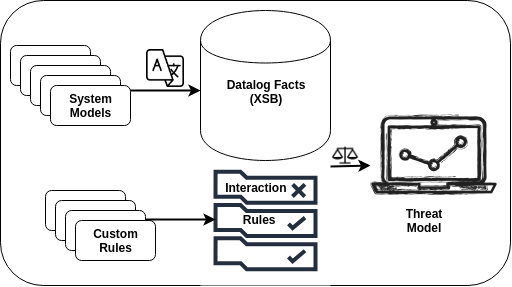
\includegraphics[width=.5\linewidth]{img/Ptah_archs.png}
\caption{Preprocessing and Transformation Handlers (\textbf{PTaH})}
\label{fig:automation:ptah_arch}
\end{figure} 

In metrics that compute aggregates, ratios, or simple statistics from findings and system facts, preprocessing steps may be minimal or bypassed entirely. In more complex metrics, such as those which consider the relationships between components or vulnerabilities, it may be necessary to craft the inputs expected from some composition of system facts along with some composition or chain of metric dependencies. In particular, metrics based on attack graphs and attack nets tend to make assumptions about the input structure which can be managed in this layer. We create these structures, score transitions, apply weights and mappings, and perform any other manipulations of our knowledge base in this layer to adhere to the input assumptions of particular metrics in this layer. 

% In order to experiment with different network architectures and exploit effects, it was necessary to reproduce each step in the process: 
% Install AG suite (MulVal, XSB) $\rightarrow$ Define AG input model (Datalog/Prolog) $\rightarrow$ Generate AG (Java, C++, ANTLR4, sed) $\rightarrow$ Import NVD (JSON, XML $\rightarrow$ SQL) $\rightarrow$ Implement custom adaptor for Stochastic Model expected input (Python, inference) $\rightarrow$ Insert transition matrix into provided R script (ctrl+c, ctrl+v) 
% After following this process precisely 2 times we understood why the AG based analytics community isn’t larger. Our immediate solution was to create a set of ansible roles and plays to automate the environment setup, test execution, and results collection entirely with a single command. This in itself lowers the barrier to entry for anyone interested in experimenting with attack graphs or looking to (quickly) reproduce our results.

% \begin{figure}[ht]
% 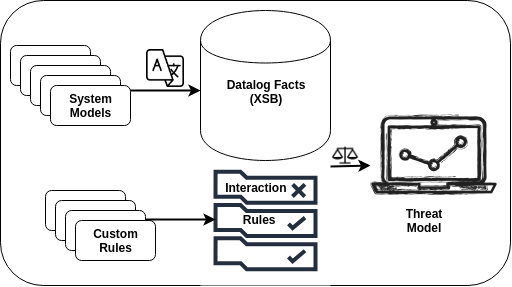
\includegraphics[width=.48\textwidth]{img/Ptah_archs.png}
% \caption{Preprocessing and Transformation Handlers (\textbf{PTaH})}
% \label{fig:automation:ptah_arch}
% \end{figure} 


% To handle the scale and volume of requests needed to support the advanced use-cases listed below, we are currently implementing and evaluating the following features in the SMaaS architecture:
% Metric Isolation: Each metric should be independently deployable to allow scaling up and down as request volume dictates. Currently metrics are bundled in Python and R modules with logical separation at the function level.




